\input{preambulo_presentacion_Berlin_beaver}
\usepackage{pifont}
\usepackage{siunitx}
\newcommand{\cmark}{\ding{51}}%
\newcommand{\xmark}{\ding{55}}%
\definecolor{cadmiumgreen}{rgb}{0.0, 0.42, 0.24}
\makeatletter
\setbeamertemplate{footline}
{
  \leavevmode%
  \hbox{%
  \begin{beamercolorbox}[wd=.333333\paperwidth,ht=2.25ex,dp=1ex,center]{section in foot}%
    \usebeamerfont{section in foot} \insertsection
  \end{beamercolorbox}%
  \begin{beamercolorbox}[wd=.333333\paperwidth,ht=2.25ex,dp=1ex,center]{subsection in foot}%
    \usebeamerfont{subsection in foot}  \insertsubsection
  \end{beamercolorbox}%
  \begin{beamercolorbox}[wd=.333333\paperwidth,ht=2.25ex,dp=1ex,right]{date in head/foot}%
    \usebeamerfont{date in head/foot} \insertshortdate{} \hspace*{2em}
    \insertframenumber{} / \inserttotalframenumber \hspace*{2ex} 
  \end{beamercolorbox}}%
  \vskip0pt%
}
\makeatother
%--------------------------------------------------------------------
%--------------------------------------------------------------------
\newcounter{choice}
\renewcommand\thechoice{\Alph{choice})}
%\newcommand\choicelabel{\thechoice.}
\newcommand\choicelabel{\thechoice}

\newenvironment{choices}%
  {\list{\choicelabel}%
     {\usecounter{choice}\def\makelabel##1{\hss\llap{##1}}%
       \settowidth{\leftmargin}{W.\hskip\labelsep\hskip 2.5em}%
       \def\choice{%
         \item
       } % choice
       \labelwidth\leftmargin\advance\labelwidth-\labelsep
       \topsep=0pt
       \partopsep=0pt
     }%
  }%
  {\endlist}

\newenvironment{oneparchoices}%
  {%
    \setcounter{choice}{0}%
    \def\choice{%
      \refstepcounter{choice}%
      \ifnum\value{choice}>1\relax
        \penalty -50\hskip 1em plus 1em\relax
      \fi
      \choicelabel
      \nobreak\enskip
    }% choice
    % If we're continuing the paragraph containing the question,
    % then leave a bit of space before the first choice:
    \ifvmode\else\enskip\fi
    \ignorespaces
  }%
  {}
%----------------------------------------------------------
%----------------------------------------------------------

\setbeamertemplate{navigation symbols}{}
\date{18 de marzo de 2021}
\title{Sesión 3. Razonamiento matemático}
\subtitle{Asesoría}
\begin{document}
\maketitle
\fontsize{14}{14}\selectfont
\spanishdecimal{.}
\section*{Contenido}
\frame[allowframebreaks]{\tableofcontents[currentsection, hideallsubsections]}
\section{Habilidad matemática}
\frame{\tableofcontents[currentsection, hideothersubsections]}

\subsection{Batería de ejercicios}

\begin{frame}
\frametitle{Ejercicio 1}
Observa la siguiente lista de números:
\begin{align*}
2, \, 6, \, 4, \, 8, \, 6, \, 10, \, \ldots
\end{align*}
¿Qué número ocupa el lugar $31$?
\begin{choices}
\choice $62$ \\
\choice $32$ \\
\choice $31$ \\
\choice $30$ \\
\choice $28$
\end{choices}
\pause
\begin{tikzpicture}[overlay]
    \node [text = cadmiumgreen] at (1, 3.3) {\cmark};
\end{tikzpicture}
\end{frame}
\begin{frame}
\frametitle{La secuencia para los $n$ pares e impares}
Tenemos que:
\begin{align*}
2, \, 6, \, 4, \, 8, \, 6, \, 10, \, \ldots
\end{align*}
\begin{tikzpicture}[overlay]
  \node at (2, 0.5) {$n =$};
  \node at (3.5, 0.5) {$1$};
  \node at (4, 0.5) {$2$};
  \node at (4.6, 0.5) {$3$};
  \node at (5.1, 0.5) {$4$};
  \node at (5.7, 0.5) {$5$};
  \node at (6.3, 0.5) {$6$};
\end{tikzpicture}
\end{frame}
\begin{frame}
\frametitle{Patrón para las posiciones pares e impares}
De la sucesión:
\begin{align*}
2, \, 6, \, 4, \, 8, \, 6, \, 10, \, \ldots
\end{align*}
\begin{tikzpicture}[overlay]
    \node at (2, 0.5) {$n =$};
    \node at (3.5, 0.5) {$1$};
    \node at (4, 0.5) {$2$};
    \node at (4.6, 0.5) {$3$};
    \node at (5.1, 0.5) {$4$};
    \node at (5.7, 0.5) {$5$};
    \node at (6.3, 0.5) {$6$};
\end{tikzpicture}
\\
\bigskip
\pause
Veamos qué relación guardan aquellos números que están en las posiciones impares y pares.
\end{frame}
\begin{frame}
\frametitle{Patrón posiciones impares}
\begin{align*}
2, \, 6, \, 4, \, 8, \, 6, \, 10, \, \ldots
\end{align*}
\begin{tikzpicture}[overlay]
    \node at (2, 0.5) {$n =$};
    \node at (3.5, 0.5) {$1$};
    %\node at (4, 0.5) {$2$};
    \node at (4.6, 0.5) {$3$};
    %\node at (5.1, 0.5) {$4$};
    \node at (5.7, 0.5) {$5$};
    %\node at (6.3, 0.5) {$6$};
\end{tikzpicture}
\\
\bigskip
\pause
El patrón que relaciona la posición $n$ impar con el valor en la sucesión es:
\pause
\begin{align*}
n + 1
\end{align*}
\end{frame}
\begin{frame}
\frametitle{Patrón posiciones pares}
\begin{align*}
2, \, 6, \, 4, \, 8, \, 6, \, 10, \, \ldots
\end{align*}
\begin{tikzpicture}[overlay]
    \node at (2, 0.5) {$n =$};
    %\node at (3.5, 0.5) {$1$};
    \node at (4, 0.5) {$2$};
    %\node at (4.6, 0.5) {$3$};
    \node at (5.1, 0.5) {$4$};
    %\node at (5.7, 0.5) {$5$};
    \node at (6.3, 0.5) {$6$};
\end{tikzpicture}
\\
\bigskip
\pause
El patrón que relaciona la posición $n$ par con el valor en la sucesión es:
\pause
\begin{align*}
n + 4
\end{align*}
\end{frame}
\begin{frame}
\frametitle{Resumen}
Se tiene entonces que:
\begin{align*}
\mbox{para } &n \mbox{ impar} \rightarrow n + 1 \\[0.5em]
\mbox{para } &n \mbox{ par} \rightarrow n + 4
\end{align*}
\\
\bigskip
\pause
Entonces para el valor que nos pide el enunciado de $n = 31$, se tiene que:
\pause
\begin{align*}
31 + 1 = 32
\end{align*}
Que corresponde al inciso \textbf{B)}
\end{frame}
\begin{frame}
\frametitle{Ejercicio 2}
Observa la siguiente lista de números y letras:
\begin{align*}
2 \, a \,  b, 6 \, b \, c, 10 \, c \, d, \ldots
\end{align*}
¿Qué lugar ocupa el número y letras: $26 \, g \, h$
\begin{choices}
\choice $6$ \\
\choice $5$ \\
\choice $7$ \\
\choice $8$ \\
\choice $10$
\end{choices}
\pause
\begin{tikzpicture}[overlay]
    \node [text = cadmiumgreen] at (1, 4.1) {\cmark};
\end{tikzpicture}
\end{frame}
\begin{frame}
\frametitle{Ejercicio 3}
El número $657$ ¿Qué lugar ocupa en la siguiente secuencia?
\begin{align*}
012, \, 123, \, \ldots, \, 890, \, 901, \, 012
\end{align*}
\begin{choices}
\choice $3$ \\
\choice $5$ \\
\choice No está en la secuencia \\
\choice $10$ \\
\choice $7$
\end{choices}
\pause
\begin{tikzpicture}[overlay]
    \node [text = cadmiumgreen] at (1, 2.6) {\cmark};
\end{tikzpicture}
\end{frame}
\begin{frame}
\frametitle{Ejercicio 4}
¿Cuál es el patrón numérico de la sucesión numérica? ($n$ es la posición en la sucesión)
\begin{align*}
2, \, 6, \, 10, \, 14, \, 18, \ldots, v
\end{align*}
\begin{choices}
\choice $v = n + 2$ \\
\choice $v = n + 3$ \\
\choice $v = 2 \, n + 4$ \\
\choice $v = 4 \, n - 2$ \\
\choice $v = 4(n + 2)$
\end{choices}
\pause
\begin{tikzpicture}[overlay]
    \node [text = cadmiumgreen] at (1, 1.7) {\cmark};
\end{tikzpicture}
\end{frame}
\begin{frame}
\frametitle{Detalle de la solución}
En este ejercicio hay que ocupar tanto el valor $v$ en la sucesión como la posición $n$, para entonces determinar el patrón.
\end{frame}
\begin{frame}
\frametitle{Detalle de la solución}
Tenemos entonces:
\pause
\begin{align*}
2, \, 6, \, 10, \, 14, \, 18, \ldots, v
\end{align*}
\begin{tikzpicture}[overlay]
    \node at (2, 0.5) {$n = $};
    \node at (3.3, 0.5) {$1$};
    \node at (3.8, 0.5) {$2$};
    \node at (4.5, 0.5) {$3$};
    \node at (5.3, 0.5) {$4$};
    \node at (6.1, 0.5) {$5$};
\end{tikzpicture}
\pause
\\
\bigskip
El paso que hay que realizar es determinar la relación entre $v$ y $n$.
\end{frame}
\begin{frame}
\frametitle{Sustituyendo en las expresiones}
La manera más rápida para encontrar la respuesta correcta, es evaluar la expresión que se nos da en cada inciso, y ver si recuperamos los primeros términos de la sucesión.
\end{frame}
\begin{frame}
\frametitle{Sustituyendo en las expresiones}
\begin{align*}
2, \, 6, \, 10, \, 14, \, 18, \ldots, v
\end{align*}
\begin{tikzpicture}[overlay]
    \node at (2, 0.5) {$n = $};
    \node at (3.3, 0.5) {$1$};
    \node at (3.8, 0.5) {$2$};
    \node at (4.5, 0.5) {$3$};
    \node at (5.3, 0.5) {$4$};
    \node at (6.1, 0.5) {$5$};
\end{tikzpicture}
\pause
\\
\bigskip
Comenzamos con el inciso \textbf{A):} $n + 2$:
\pause
\begin{eqnarray*}
1 + 2 = 3, \pause 2 + 2 = 4 
\end{eqnarray*}
\pause
Claramente este patrón no nos devuelve los primeros dos términos de la sucesión, por lo tanto, no es correcto.
\end{frame}
\begin{frame}
\frametitle{Sustituyendo en las expresiones}
\begin{align*}
2, \, 6, \, 10, \, 14, \, 18, \ldots, v
\end{align*}
\begin{tikzpicture}[overlay]
    \node at (2, 0.5) {$n = $};
    \node at (3.3, 0.5) {$1$};
    \node at (3.8, 0.5) {$2$};
    \node at (4.5, 0.5) {$3$};
    \node at (5.3, 0.5) {$4$};
    \node at (6.1, 0.5) {$5$};
\end{tikzpicture}
\pause
\\
\bigskip
Ocupamos el inciso \textbf{B):} $n + 4$:
\pause
\begin{eqnarray*}
1 + 4 = 5, \pause 2 + 4 = 6 
\end{eqnarray*}
\pause
Este patrón no nos devuelve los primeros dos términos de la sucesión, por lo tanto, no es correcto.
\end{frame}
\begin{frame}
\frametitle{Sustituyendo en las expresiones}
\begin{align*}
2, \, 6, \, 10, \, 14, \, 18, \ldots, v
\end{align*}
\begin{tikzpicture}[overlay]
    \node at (2, 0.5) {$n = $};
    \node at (3.3, 0.5) {$1$};
    \node at (3.8, 0.5) {$2$};
    \node at (4.5, 0.5) {$3$};
    \node at (5.3, 0.5) {$4$};
    \node at (6.1, 0.5) {$5$};
\end{tikzpicture}
\pause
\\
\bigskip
Ahora vamos con el inciso \textbf{C):} $2 \, n + 4$:
\pause
\begin{eqnarray*}
2 (1) + 4 = 6, \pause \hspace{0.3cm} 2(2) + 4 = 8 
\end{eqnarray*}
\pause
Este patrón tampoco nos devuelve los primeros dos términos de la sucesión, por lo tanto, no es correcto.
\end{frame}
\begin{frame}
\frametitle{Sustituyendo en las expresiones}
\begin{align*}
2, \, 6, \, 10, \, 14, \, 18, \ldots, v
\end{align*}
\begin{tikzpicture}[overlay]
    \node at (2, 0.5) {$n = $};
    \node at (3.3, 0.5) {$1$};
    \node at (3.8, 0.5) {$2$};
    \node at (4.5, 0.5) {$3$};
    \node at (5.3, 0.5) {$4$};
    \node at (6.1, 0.5) {$5$};
\end{tikzpicture}
\pause
\\
\bigskip
Comenzamos con el inciso \textbf{D):} $4 \, n - 2$:
\pause
\begin{eqnarray*}
4(1) - 2 = 2, \pause 4(2) - 2 = 6 
\end{eqnarray*}
\pause
Este patrón nos devuelve los primeros dos términos de la sucesión, por lo tanto, es el \textbf{inciso correcto}.
\end{frame}
\begin{frame}
\frametitle{Ejercicio 5}
¿Qué número falta en el espacio vacío para que los números sigan un mismo patrón?
\\
\bigskip
\begin{minipage}{0.4\linewidth}
\begin{figure}[H]
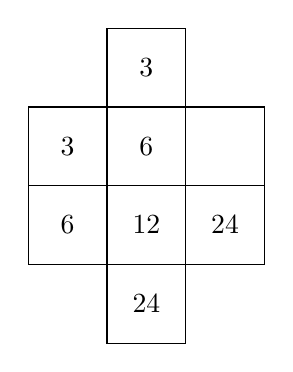
\begin{tikzpicture}
  \draw (0, 0) rectangle (1, 1) node [pos=0.5] {$24$};
  \draw (0, 1) rectangle (1, 2) node [pos=0.5] {$12$};
  \draw (-1, 1) rectangle (0, 2) node [pos=0.5] {$6$};
  \draw (-1, 2) rectangle (0, 3) node [pos=0.5] {$3$};
  \draw (1, 2) rectangle (2, 3);
  \draw (1, 1) rectangle (2, 2) node [pos=0.5] {$24$};
  \draw (0, 2) rectangle (1, 3) node [pos=0.5] {$6$};
  \draw (0, 3) rectangle (1, 4) node [pos=0.5] {$3$};
\end{tikzpicture}
\end{figure}
\end{minipage}
\hspace{1cm}
\begin{minipage}{0.4\linewidth}
\begin{tabular}{l l}
A) & $18$ \\
B) & $6$ \\
C) & $12$ \\
D) & $3$ \\
E) & $24$ \\
\end{tabular}
\pause
\begin{tikzpicture}[overlay]
    \node [text = cadmiumgreen] at (-2.1, 0.2) {\cmark};
\end{tikzpicture}
\end{minipage}  
\end{frame}
\begin{frame}
\frametitle{Ejercicio 6}
¿Qué tipo de patrón numérico se observa en la siguiente secuencia?
\begin{align*}
144, \, 121, \, 100, \, 81, \, 64
\end{align*}
\begin{choices}
\choice Aumenta la raíz consecutivamente \\
\choice Disminuye la raíz consecutivamente \\
\choice Disminuye consecutivamente el exponente \\
\choice Aumenta el exponente de la potencia \\
\choice Disminuye la base de la potencia.
\end{choices}
\pause
\begin{tikzpicture}[overlay]
    \node [text = cadmiumgreen] at (1, 1) {\cmark};
\end{tikzpicture}
\end{frame}
\begin{frame}
\frametitle{Ejercicio 7}
A Daniel, David y Darío les dieron 360 canicas, se repartieron de la siguiente forma: a Darío le dieron $\frac{1}{4}$ del total, a David le dieron $\frac{1}{3}$ del total, ¿cuántas canicas le dieron a Daniel?
\begin{choices}
\choice $90$ \\
\choice $120$ \\
\choice $150$ \\
\choice $200$ \\
\choice $220$
\end{choices}
\pause
\begin{tikzpicture}[overlay]
    \node [text = cadmiumgreen] at (1, 2.5) {\cmark};
\end{tikzpicture}
\end{frame}
\begin{frame}
\frametitle{Ejercicio 8}
De un premio de $\$300$, Fernando se quedó con $\$55$, Alejandro con el triple de Fernando, y Daniel con el resto. ¿Con cuánto se quedó Daniel?
\begin{choices}
\choice $\$35$
\choice $\$105$ \\
\choice $\$155$ \\
\choice $\$90$ \\
\choice $\$80$ \\
\end{choices}
\pause
\begin{tikzpicture}[overlay]
    \node [text = cadmiumgreen] at (1, 1) {\cmark};
\end{tikzpicture}
\end{frame}
\begin{frame}
\frametitle{Ejercicio 8}
La suma de las edades de Rosario y Ángeles es de $50$ años. Si Rosario es $6$ años mayor que Ángeles, ¿qué edad tiene Ángeles?
\begin{choices}
\choice $28$
\choice $18$ \\
\choice $22$ \\
\choice $26$ \\
\choice $16$ \\
\end{choices}
\pause
\begin{tikzpicture}[overlay]
    \node [text = cadmiumgreen] at (1, 2.6) {\cmark};
\end{tikzpicture}
\end{frame}
\begin{frame}
\frametitle{¿Por qué es correcto?}
Este enunciado ya nos exige un esfuerzo mayor, ya que lo que tenemos que hacer, es plantear una ecuación para obtener la edad de Ángeles.
\\
\bigskip
\pause
Veamos a continuación la manera de expresar la ecuación.
\end{frame}
\begin{frame}
\frametitle{La ecuación de las edades}
La edad de Rosario es $R$ y la edad de Ángeles es $A$.
\\
\bigskip
El enunciado primero nos dice que \emph{La suma de las edades de Rosario y Ángeles es de $50$ años.}, es decir:
\begin{align*}
R + A =  50
\end{align*}
\pause
Luego nos dice el enunciado que: \emph{Rosario es 6 años mayor que Ángeles.}
\end{frame}
\begin{frame}
\frametitle{La ecuación de las edades}
Entonces, podemos expresar la ecuación inicial en términos de la edad de Ángeles, es decir;
\pause
\begin{eqnarray*}
R + A &=& 50 \\[0.25em] \pause
(A + 6) + A &=& 50 \\[0.25em] \pause
2 \, A + 6 &=& 50 \\[0.25em] \pause
2 \, A &=& 50 - 6 \\[0.25em] \pause
2 \, A &=& 44 \\[0.25em] \pause
A &=& 22
\end{eqnarray*}
\end{frame}
\begin{frame}
\frametitle{Comprobando el resultado}
Al haber obtenido la edad de Ángeles que corresponde al inciso \textbf{C)}, podemos obtener la edad de Rosario:
\pause
\begin{eqnarray*}
R + A &=& 50 \\[0.25em]
R + 22 &=& 50 \\[0.25em]
R &=& 50 - 22 \\[0.25em]
R &=& 28
\end{eqnarray*}
\pause
De tal manera que la suma de las dos edades, es de $50$ años.
\end{frame}
\begin{frame}
\frametitle{Ejercicio 9}
La mitad de $\dfrac{3}{4}$ es:
\begin{choices}
\choice $\frac{1}{8}$
\choice $\frac{1}{2}$ \\
\choice $\frac{3}{6}$ \\
\choice $\frac{3}{8}$ \\
\choice $\frac{6}{8}$ \\
\end{choices}
\pause
\begin{tikzpicture}[overlay]
    \node [text = cadmiumgreen] at (1, 1.8) {\cmark};
\end{tikzpicture}
\pause
\begin{tikzpicture}[overlay]
  \node at (8, 4) {$\dfrac{3}{4}$}; \pause
  \node at (8, 3.3) {$\_\_$};
  \node at (8, 2.8) {$2$}; \pause
  \draw [fill=white, white] (7.8, 2.6) rectangle (8.2, 3); \pause
  \node at (8, 2.6) {$\dfrac{2}{1}$}; \pause
  \draw [thick, blue] (7.6, 2.2) -- (7.2, 2.2) -- (7.2, 4.3) -- (7.6, 4.3); \pause
  \draw [thick, red] (8.4, 2.9) -- (8.8, 2.9) -- (8.8, 3.6) -- (8.4, 3.6); \pause
  \node at (9.5, 3.3) {$=\dfrac{3}{8}$};
\end{tikzpicture}
\end{frame}
\begin{frame}
\frametitle{Ejercicio 10}
Raúl cumplirá $16$ años dentro de 7 meses.
\medskip
¿Cuántos meses faltan para que cumpla dieciocho años y medio?
\begin{choices}
\choice $35$
\choice $37$ \\
\choice $24$ \\
\choice $31$ \\
\choice $38$ \\
\end{choices}
\pause
\begin{tikzpicture}[overlay]
    \node [text = cadmiumgreen] at (1, 3.5) {\cmark};
\end{tikzpicture}
\end{frame}
\begin{frame}
\frametitle{Ejercicio 11}
La suma de $2$ números es $12$ y su diferencia $6$, ¿cuáles son esos números?
\begin{choices}
\choice $7,\, 5$
\choice $8 \, 4$ \\
\choice $10, \, 2$ \\
\choice $9, \, 3$ \\
\choice $11, \, 1$ \\
\end{choices}
% \pause
% \begin{tikzpicture}[overlay]
%     \node [text = cadmiumgreen] at (1, 1.7) {\cmark};
% \end{tikzpicture}
\end{frame}
\begin{frame}
\frametitle{Otro tipo de ejercicio}
Este ejercicio plantea dos premisas en el enunciado:
\setbeamercolor{item projected}{bg=blue!70!black,fg=yellow}
\setbeamertemplate{enumerate items}[circle]
\begin{enumerate}[<+->]
\item La suma de $2$ números es $12$.
\item Y su diferencia es $6$.
\end{enumerate}
\pause
Entonces tendremos que plantear de alguna manera la informción que nos están dando.
\\
\bigskip
\pause
Tendremos que apoyarnos con el \emph{álgebra}.
\end{frame}
\begin{frame}
\frametitle{La primera premisa}
Llamemos a los dos números como $a$ y $b$.
\pause
Entonces la primera premisa nos dice: \enquote{La suma de $2$ números es $12$}.
\pause
Que expresamos como:
\begin{align*}
a + b =  12
\end{align*}
\end{frame}
\begin{frame}
\frametitle{la segunda premisa}
Como ya hemos nombrado a los dos número como $a$ y $b$, expresos la segunda premisa: \enquote{y su diferencia es $6$}. Quedando como:
\begin{align*}
a - b =  6
\end{align*}
\pause
El siguiente paso es juntar las dos premisas.
\end{frame}
\begin{frame}
\frametitle{Sistema de ecuaciones}
Tenemos entonces un sistema de dos ecuaciones que involucran a los dos números:
\begin{align*}
a + b &= 12 \\[0.5em]
a - b &= 6
\end{align*}
Es un sistema de dos ecuaciones con dos incógnitas.
\end{frame}
\begin{frame}
\frametitle{Solución al sistema simultáneo}
Este sistema simultáneo se resuelve de la siguiente manera: consideramos una incógnita ya sea $a$ o $b$, para encontrar un valor.
\\
\bigskip
\pause
Una vez que hemos encontrado el valor de la primera incógnita, lo ocupamos para calcular la segunda.
\end{frame}
\begin{frame}
\frametitle{Eligiendo una incógnita}
Escogemos la primera incógnita: $a$, vemos que del sistema de ecuaciones, si sumamos la primera ecuación con la segunda tenemos:
\begin{align*}
a + b &= 12 \\
a - b &= 6 \\[-11pt]
\cline{1-2} 
2 \, a + 0 &= 18
\end{align*}
\pause
Entonces: $2 \, a =  18$. \hspace{1.5cm} \pause Así: $a = 9$.
\end{frame}
\begin{frame}
\frametitle{Ocupando el resultado para la otra incógnita}
Con el resultado que encontramos, podemos obtener la segunda incógnita, al sustituir el valor de $a$ en cualquiera de las dos ecuaciones, tomemos la primera:
\pause
\begin{eqnarray*}
a + b &=& 12 \\ \pause
9 + b &=& 12 \\ \pause
b &=& 12 - 9 \\ \pause
b &=& 3
\end{eqnarray*}
\pause
Por tanto los valores son $a = 6$ y $b = 3$, que corresponden al inciso \textbf{D)}.
\end{frame}
\begin{frame}
\frametitle{Ejercicio 11}
La suma de $2$ números es $12$ y su diferencia $6$, ¿cuáles son esos números?
\begin{choices}
\choice $7,\, 5$
\choice $8 \, 4$ \\
\choice $10, \, 2$ \\
\choice $9, \, 3$ \\
\choice $11, \, 1$ \\
\end{choices}
\begin{tikzpicture}[overlay]
    \node [text = cadmiumgreen] at (1, 1.7) {\cmark};
\end{tikzpicture}
\end{frame}
\begin{frame}
\frametitle{Ejercicio 12}
Si el diámetro de un círculo mide $\SI{10}{\meter}$, ¿cuánto mide el radio?:
\begin{choices}
\choice $\SI{0.500}{\meter}$
\choice $\SI{5}{\meter}$ \\
\choice $\SI{0.50}{\meter}$ \\
\choice $\SI{0.5}{\meter}$ \\
\choice $\SI{0.005}{\meter}$ \\
\end{choices}
\pause
\begin{tikzpicture}[overlay]
    \node [text = cadmiumgreen] at (1, 3.5) {\cmark};
\end{tikzpicture}
\end{frame}
\begin{frame}
\frametitle{Ejercicio 13}
Un plomero tiene un tubo de $\SI{10}{\meter}$, si a diario corta un tramo de $\SI{2}{\meter}$, terminará de cortarlo en:
\medskip
\begin{choices}
\choice $2$ días
\choice $3$ días \\
\choice $4$ días \\
\choice $5$ días \\
\choice $6$ días \\
\end{choices}
\pause
\begin{tikzpicture}[overlay]
    \node [text = cadmiumgreen] at (1, 2.6) {\cmark};
\end{tikzpicture}
\end{frame}
\begin{frame}
\frametitle{Ejercicio 14}
Si el área de un cuadrado es de $\SI{121}{\square\meter}$, ¿Cuál es su perímetro?
\medskip
\begin{choices}
\choice $\SI{11}{\meter}$
\choice $\SI{22}{\meter}$ \\
\choice $\SI{44}{\meter}$ \\
\choice $\SI{121}{\meter}$ \\
\choice $\SI{40}{\meter}$ \
\end{choices}
\pause
\begin{tikzpicture}[overlay]
    \node [text = cadmiumgreen] at (1, 2.6) {\cmark};
\end{tikzpicture}
\end{frame}
\end{document}